\documentclass[paper=a4, fontsize=11pt]{scrartcl}

\usepackage[utf8]{inputenc}
\usepackage{fourier} % Adobe Utopia
\usepackage[english]{babel}
\usepackage{amsmath,amsfonts,amsthm}
\usepackage{relsize}
\usepackage[acronym,toc]{glossaries}
\usepackage{svg}
\usepackage{enumitem}
\usepackage{nameref}
\usepackage[ampersand]{easylist}
\usepackage{graphicx}

\usepackage{multicol}
\usepackage{sectsty}
\allsectionsfont{\normalfont\scshape} 

\usepackage{fancyhdr}
\pagestyle{fancyplain}
\fancyhead{}
\fancyfoot[L]{} 
\fancyfoot[C]{}
\fancyfoot[R]{\thepage}
\renewcommand{\headrulewidth}{0pt}
\renewcommand{\footrulewidth}{0pt}
\setlength{\headheight}{14.6pt}
\graphicspath{{res/}}

\usepackage{stmaryrd}
\usepackage{url}
\usepackage[section]{placeins}
\usepackage{caption}
\captionsetup{width=0.7\textwidth}

\usepackage{hyperref}
\hypersetup{colorlinks,
    citecolor=black,
    filecolor=black,
    linkcolor=black,
    urlcolor=black
}

\newcommand{\horrule}[1]{\rule{\linewidth}{#1}}
\hoffset = -0pt
\voffset = -20pt
\textwidth = 450pt
\textheight = 700pt

\title{%
    \normalfont{}
    \normalsize{}
    \textsc{École nationale supérieure d'informatique et de mathématiques appliquées de Grenoble} \\ [10pt]
    \horrule{0.5pt} \\[0.4cm]
    \huge Prototyping a massively multiplayer game server
    \horrule{2pt} \\[0.5cm]
}

\author{Yann COLINA\\
Bastien ETCHEGOYEN\\
Etienne L'HER\\
Floran NARENJI-SHESHKALANI} 

\date{\normalsize\today}

\newacronym{MMO}{MMORPG}{massively multiplayer online role playing game}
% \newacronym{WoW}{WoW}{World of Warcraft}
\newacronym{NPC}{NPC}{Non playing characters}

\begin{document}

\maketitle

\iffalse{}
* Reflection
* Actor system/hierarchy
* API
* Diagrams
    * Actors hierarchy/messages
    * Client protocol
* Protocol (scodec)
* Handlers
* AuthServer
    * SRP6a
* WorldServer
    * RC4a
    * Actor interactions (EventStream)
* Reverse engineering difficulties
    * Big protocol, organicly built, too many features
* Sources
    * TrinityCore
    * Akka docs
    * Scala docs
    * scodec
* Scala
    * Functional
    * Immutable
    * Preferred language for Akka actors (ugly in Java)
    * Strongly typed
    * Full of syntaxic sugar
    * Ahead of its time ('research language')
    * Home grown language (der Schweiz)

\fi

\pagebreak
\tableofcontents
\pagebreak

\section{Introduction}

This project was an experiment in writing a server for an online
video game.
The academic goal was to get hands-on experience about designing and building a
complex server from scratch, without missing any aspects of it: from basic blocks
such as networking, cryptography and concurrency to managing the world itself.

This project was done as a part of the Ensimag's second year module `Specialty
project'.
The idea was at the initiative of the students.

The source code under MIT license is available at
\url{https://github.com/SKNZ/EnsiWoW}.

\subsection{World of Warcraft}

For such a purpose, we chose the World of Warcraft video game.
Indeed, writing our own video game client would have been both out of the scope
of this project and, in terms of time spent, mutually exclusive with writing the
server for it.
Moreover, the video game sector has by nature little to no available open source
game clients that would fit the purpose of this project.
Consequently, it was decided to settle on an existing video game.

With prior knowledge and additional research, World of Warcraft was determined
to be the video game for which writing a server would be most interesting: being
the most popular and populous game of its type for the last decade, the
technical aspects were certain to be production grade.
Furthermore, the protocol is well documented and there exists very advanced open
source implementations of it.

\begin{figure}[htb!]
    \centering
    
\includegraphics[width=0.5\textwidth]{wow}
\end{figure}

\FloatBarrier{}

\subsubsection{Disclaimer}

World of Warcraft is proprietary software.
Regular players pay a monthly subscription fee.
This project is only done as a learning experience, by students in a fully
academic context.
In other words, this is a research project with no goals whatsoever towards
facilitating copyright infringement.

This project is under the MIT license, as found in the repository's root folder.

\subsection{General information about MMORPGs}

MMORPGs are exclusively online video games: without a network connection, the
game cannot be played. Unlike more traditional games such as first-person
shooters, the players evolve in a fully shared persistent open world.

In these games, the server is authoritative: in real time, each player tells of
its actions to the server, which authorizes them and then sends out the
information to the other players (for example, players will be informed when a
nearby players attack a creature).
In terms of network topology, this model is known as the star model, in which
every communication goes through a central server.

On a non-technical note, for the players of such game, the goals are often about
creating a character and making it stronger, e.g.\ by fighting creatures and
gaining equipment.

\subsection{Stated objectives}

This project was done as a part of the Ensimag's module named `Specialty
project'.
With World of Warcraft's development budget numbering in millions of dollars and
a single semester of classes at our disposal, it was obvious that only a minimal
subset of features from the original game server could be implemented.\

The features to be implemented are:
\begin{itemize}
    \item Authentication
    \item Realm selection
    \item Character management
    \item Joining the world
    \item Movement
    \item Seeing other players actions
\end{itemize}

While all these features are extremely basic and are all-together insufficient
for anyone to consider seriously playing the game, they did provide enough work
to last until the end of the project.

\subsection{TrinityCore}

TrinityCore is an open source project for a game server that is compatible with
the World of Warcraft client.
Unlike our implementation, their codebase is nearly 13 years old (through many
forks) and provides a playing experience that is much closer, but certainly
inferior, to the official experience.

The reverse engineering work was primarily done by this project and its
predecessors, which is why we felt it was important to give them a special
mention here.\\

However, a codebase that is as old as TrinityCore is bound to have some
flaws. Indeed, modern considerations, for example on distributed systems,
scalability or open source code base management, did not exist when most of the
work on TrinityCore was done.

Though TrinityCore was indeed an inspiration for this project, our goal is not
to simply translate code from C++ to Scala.
With the usage of Scala and Akka actors, we intend to have a scalable and
eventually distributed solution with a clean and hopefully elegant codebase.

% \clearpage

\section{Building blocks of a World of Warcraft game server}

\subsection{Actors}

An actor is the basic computational unit of an actor system.

An actor follows a few axioms:
\begin{itemize}
    \item An actor can send a message to another actor
    \item An actor can create a child actor
    \item An actor's received messages are stored in a mailbox and processed one
        at a time
    \item An actor can have mutable data only if it is private
    \item Messages exchanged by actors should contain only immutable data
\end{itemize}

The lack of mutable shared state makes actors a way to express concurrent
problems elegantly without wrestling directly with synchronization primitives.

As with most good coding practices, actors should have a single responsibility.
Therefore, actors should be lightweight and cost very little to make.
In practice, actor systems are made to handle enormous number of actors, meaning
that actors are not implemented as system threads. Often times, actors are
scheduled atop a thread pool.\\

For the purpose of writing a World of Warcraft game server, and more generally
an MMORPG game server, actors have an obvious appeal: each entity of the world
could be represented as an actor.
Interactions between entities would then be simple message exchanges.

There is no knowledge of how such a system would behave in practice: actors
have an overhead, and having one actor per world entity might be too much.
While the optimal granularity will have to be determined, it certainly will be
much finer than it would be with system threads.

% * What are actors
% * Why are they nice
% * Why would they fit well with the conception of an MMORPG

\subsection{Technological choices and project management}

We chose to write the server in Scala, using the Akka library.
Scala was an interesting choice for us, as it is a hybrid functional/imperative
language, with JVM binary compatibility and wide enough adoption.
It is a very rich language, with an extreme amount of flexibility and syntactic
sugar.

For actors, Akka is the go-to library, which is also one of the reasons we chose
Scala.

As for other libraries, we prominently used \texttt{scodec}, for our
serialization needs, and some elements of \texttt{BouncyCastle} for
cryptography.

For unit testing, we used the \texttt{scalatest} library.

On a related note, \texttt{git} (on GitHub) was our version control system of
choice.  For the duration of the project, we have adhered strictly to
peer-reviewed pull requests with necessary \texttt{TravisCI} (continuous
integration) approval before merging into master.
Task tracking was done using a Trello board.
We feel these tools bring a lot of value to the team, and encourage their usage.

\subsection{Networking}

The interface between the authentication and realm servers, and the outside
world (the clients) is managed by the \texttt{TCPServer} actors, one for each
server. 
When created, this actor binds itself to a socket using a custom IP address and
port.
Once connected, the actor spawns a \texttt{TCPHandler} actor, which itself is
configured to spawn the adequate actor for either the authentication or realm
servers.
The \texttt{TCPHandler} actor receives and emits data from the socket.

%\subsection{Database storage}

\subsection{Administration}

In order to interact and monitor the server, it has been decided that the most
flexible and adaptable solution was to implement an RESTful web service, to be
used by a remote client.
The flexibility comes from the fact that the HTTP routes are defined alongside
the targeted methods of the server, which would eventually be seamlessly
triggered by the game client or the administrative client.
Each part of the application willing to expose an API simply needs to
implemented the \texttt{API} trait.
In order to gather all the routes, the \texttt{WebServer} implements a
runtime reflection feature, which, by examining the compiled program, is able to
collects all the routes defined in the program and fuse them together.

Reflection is a powerful yet dangerous tool.
Indeed, in addition to examining and introspecting the code, it is also possible
to modify it, which could lead to unexpected behaviors, specially since there is
no compiler to ensure coherency.
Moreover, analyzing the code is a heavy operation, which, when done in runtime,
can significantly slow down the execution.
% * API and why it uses reflection (and what is refleciton, why it s dangerous
% etc).

\subsection{Unit tests}

The World of Warcraft client was written in C++, for the x86 architecture, which
uses little-endian. 
Our application run on the JVM, which uses big-endian.
The World of Warcraft client expects strict adherence to its binary format.

Writing code while juggling byte orders adds a layer of complexity, making an
already challenging task that much more difficult.
Moreover, mistakes result in no error: the client will silently ignore any
malformed packet, and wrong byte ordering will count as such.

Hence, it was required of us to have exact binary compatibility with the client.
In that regards, unit tests proved to be a most useful tool.
Using reference packets extracted from actual game communications, we were able
to write unit tests that validated the output of our serialization codecs.

As we refactored our code or gained better knowledge of the third party
libraries we were using, we made code improvements to stable
features.
Those often resulted in hard to spot mistakes, if not for unit tests.

% * Auth
%     * Protocol description
%         * Sequence diagram
%         * Actor diagram
%         * Principle of each packet
%             * with its cryptographical application
%     * Realm list building
%     * Account API
%     * AuthSession FSM

% \clearpage

\section{Authentication server}

The authentication server is the entry point to the World of Warcraft.  
Its address is shipped with the client, and its purpose is essentially to
validate the users credentials and offer the choice of realm.

\subsection{SRP Protocol}
The authentication server implements the SRP (Secure Remote Password) protocol 
in which, the client must demonstrate to the server that it knows the account's 
name and password without sending the password itself.

The first step requires the client to start the communication with the server
by providing the game's version and other parameters related to the computer. 
Alongside, it provides also the username to which the authentication program 
answers by sending a challenge, in case the previous parameters are 
authorized by the server. The following step analyzes the validity of the 
challenge's solution response, and if correct, it creates a session related to
the player.
Only then, the server will deliver the list of realms available.

\begin{figure}[htb!]
    \centering
    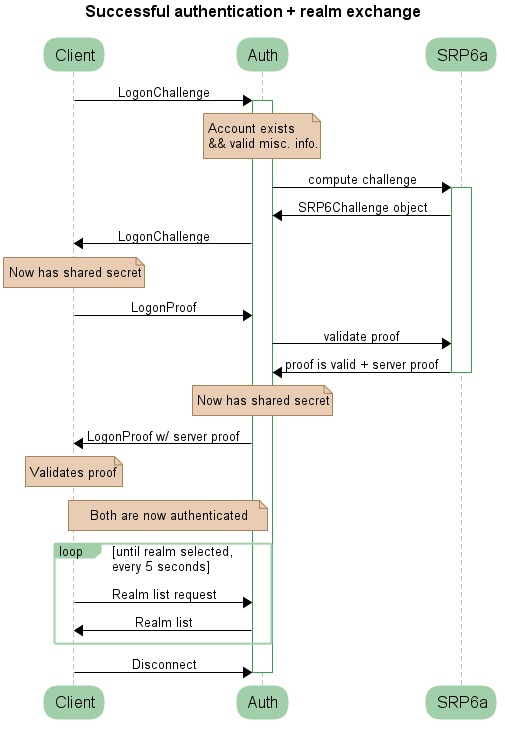
\includegraphics[width=0.7\textwidth]{authexch}
    \caption{Sequence diagram for a successful authentication/realms list
    exchange (excluding error cases)}
\end{figure}

\begin{itemize}
    \item \texttt{ClientChallenge}
        The first connection aims at checking the validity of the game's version, 
        thus, the packet contains an instance of \texttt{VersionInfo} that will 
        be analyzed and if valid, the packet's handler
        \texttt{LogonChallengeHandler} will generate a challenge

    \item \texttt{ServerLogonChallenge}
        The challenge is represented by an instance of \texttt{ServerChallenge}
        that describes the first part of an SRP6 protocol implementation. This
        object contains a key, a multiplicative group generator, a large
        prime number and a salt. It is stored in the database, associated to the
        username.

    \item \texttt{ClientLogonProof}
        In order to solve the challenge, the client generates a shared key and returns
        a client key and a proof. With this information, the server is able to generate the
        same shared key and compares the proof to the expected proof generated from the
        shared key and the client key. 

    \item \texttt{ServerLogonProof}
        Whether the expected proof is matched or not, an instance of the packet 
        \texttt{ServerLogonProof} is sent back to the client. The difference 
        is that if the user entered a valid couple username and password, the packet 
        will contain a success response code and a proof that certifies that the 
        server too has the same shared key. Otherwise, the response code will be 
        interpreted as a failed authentication.

    \item \texttt{ClientRealmlist}
        Afterwards, if the authentication succeeded, the client asks for the
        realms list

    \item \texttt{ServerRealmlist}
        The response to the request is described by an array of realms each
        defined by their nature and current state, such as the number of
        characters or the population level.

\end{itemize}

\FloatBarrier{}

\subsection{Authentication automaton}

All the while, the authentication server goes through different states and
behaviors. The packets received by the server are managed by the
\texttt{AuthSession} actor which implements a finite state machine.
The initial state, \texttt{StateNoData}, only handles logon challenges or
reconnect challenges and subsequently switches to the appropriate state.

For instance, after receiving a logon challenge, it shifts
to \texttt{StateChallenge} which analyzes the challenge request and if valid, 
sends back a challenge to the client and switches to \texttt{StateProof}. 
Otherwise, it switches to \texttt{StateFailed}.

Later on, in \texttt{StateProof}, it relays any logon proof to the appropriate
handler which eventually will send back an \texttt{EventProofSuccess} containing
the servers' logon proof.
At this point, the automaton shifts to \texttt{StateRealmlist} which, when
queried, asks the \texttt{AuthServer} actor for the available realm servers to
be sent to the client.

\begin{figure}[htb!]
    \centering
    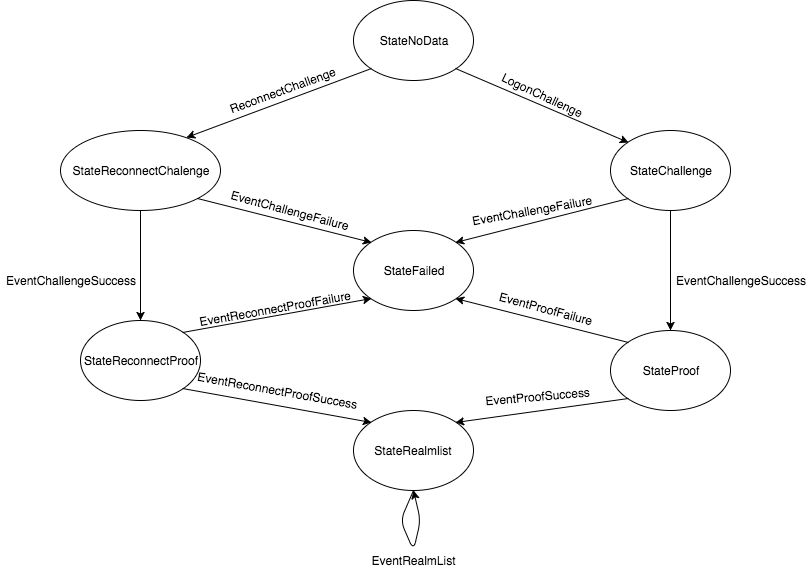
\includegraphics[width=\textwidth]{authSession}
    \caption{Authentication automaton}
\end{figure}
\subsection{Account API}

In order to interact with the database, the account management object is 
complemented by \texttt{AccountAPI} which describes different HTTP routes 
and when one of them is triggered, the appropriate account's management method is
executed. Therefore, allowing a remote and simple access to the database.

% \clearpage

\section{Realm server}

In World of Warcraft, the most basic way to split the work load is
realms.
Instead of having a single world where all players coexist, there exists many
parallel and fully isolated worlds, to the point where characters (i.e.\ a
player's progress) from one realm do not exist on another.

Once past the authentication server, the client gets a list of potential realms.
The players then selects a realm, and the client establishes a new TCP
connection to that realm server.

Similarly to the authentication server, the realm server will itself be one
actor and will instantiate other actors, most notably the TCP listener and the
packet handlers.

% * Realm
%     * Connection + cryptography
%     * Characters management
%     * World state
%         * Event stream
%     * Moving entities
%     * Concurrency stuff

\subsection{Actor hierarchy}

\begin{figure}[htb!]
    \centering
    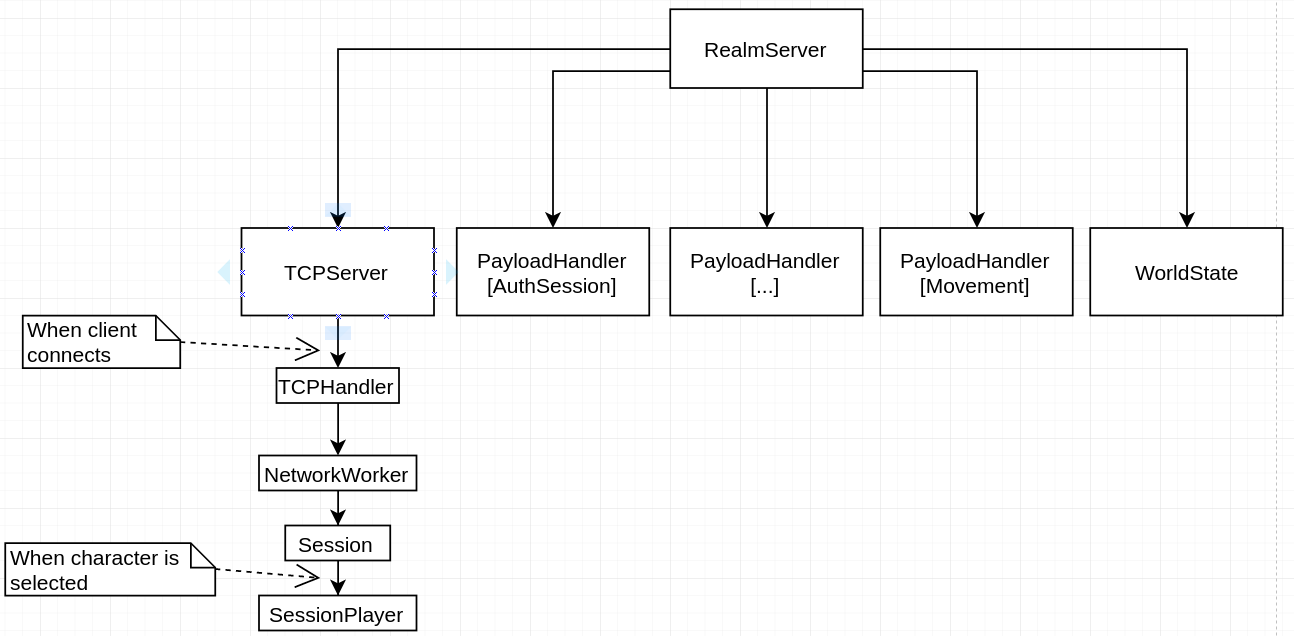
\includegraphics[width=\textwidth]{realmactors}
    \caption{Actors hierarchy for a realm server}
\end{figure}

\subsubsection{Packet handlers}

At the start of the RealmServer, using reflection (as done for the REST API),
classes implementing the \texttt{PayloadHandlerFactory} trait are instantiated
and a map associating each packet to the matching handler is built.

Once a packet has arrived to the realm server and been deserialized
successfully, its payload is passed to the correct handler.
As an example of what a handler might do, the character enumeration request
handler will load all characters for an account and build the responding packet.

Note that the packet handlers actors are by design choice fully stateless: this
has the benefit of allowing us to scale them out individually simply by adding a
load balancing actor in front of one.

\subsubsection{Client connections}

From the server side, once a TCP connection is received, a
\texttt{NetworkWorker} actor is created by the \texttt{TCPHandler} actor.
This actor's responsibility is to handle all aspects of networking for a client:
\begin{itemize}
    \item Receive incoming packets, decrypt them if applicable, deserialize them
        and pass them to the correct packet handler
    \item Serialize outgoing packets, encrypt them if applicable and send them
        over the network
\end{itemize}

The \texttt{NetworkWorker} then creates a \texttt{Session} actor, which is
responsible for maintaining all state related to the current game client.
However, it does not handle anything related to the player being in the world,
as that responsibility falls to the \texttt{SessionPlayer} actor.
The \texttt{SessionPlayer} actor will be created when the player selects a
character to play with (cf.~\ref{jtw}).

\subsubsection{Cryptography}

After the authentication server phase, the client and game server are both in
possession of a cryptographically secure random shared secret.
The client establishes a new TCP connection to the server and sends an initial
packet telling the server which account is being used for authentication.

The server retrieves the cryptographic key associated with the account from the
database.

The algorithm used in the version of protocol we support (from
2009) is RC4a (symmetric encryption) which is now known to be flawed.
The variant used in the World of Warcraft protocol skips the first 1024 bytes,
which are known to leak information.
The cipher is initialized using the shared secret.

From that point onwards, the secret is used as an encryption key for all
communications.
However, it must be noted that only the headers of every packet
(and not the contents) are encrypted.

\subsection{Characters management}

\subsubsection{Character creation}

One of the features of the realm server is the ability to create characters.
Once connected to it, the user can add a new character and choose its appearance; 
these options are transcribed in the packet \texttt{ClientCharacterCreate} that
contains:
\begin{multicols}{2}
\begin{itemize}
    \item Race
    \item Class
    \item Gender
    \item Skin tone
    \item Gender
    \item Face
    \item Hair style
    \item Hair color
    \item Facial hair
\end{itemize}
\end{multicols}

The characters creation handler tests the validity of the fields and if successful,
adds the character to a list, as well as sending a \texttt{ServerCharacterCreate}
consisting of a success response code.

\subsubsection{Characters enumeration}

When the realm server receives a payloadless packet with an opcode corresponding
to a character enumeration, \texttt{CharacterEnumHandler} sends back an instance
of \texttt{ServerCharacterEnum} which contains the array of the characters.

\subsection{World state}

\subsubsection{Event stream}

As actions in the game must be visible for other characters, there needs to
be a way to send messages to a set of players.

On the official implementation of World of Warcraft, with the expected
workloads, it would be necessary to separate the world is small subsets that have
much more workable sizes, e.g.\ by iterating only on units which are in the
players field of view.

In our simplified implementation, however, we can ignore these constraints as
our number of players is expected to be very small.\\

As a common communication channel between all actors of the world, we use Akka's
\texttt{EventStream}, which is an advanced implementation of the
publisher/subscriber pattern: it offers subscribers ability to filter on the
types of messages they want to receive.

\subsubsection{WorldState actor}

The \texttt{WorldState} actor's responsibility is to maintain knowledge about
the current state of the world.
In our case, this means:
\begin{itemize}
    \item gathering changes to the world, e.g.\ a player joining
    \item maintaining the current state of the world using those changes, e.g.\
        having a list of all players currently in the world
    \item and `ticking' the world
\end{itemize}

Ticking the world is an action that happens at a very small interval (30
milliseconds).
When the world is ticked, actions that took place during the last 30
milliseconds are grouped together and sent out to all clients in form of the
\texttt{ServerObjectUpdate} packet.
Some actions, for example movements which require more real time handling,
are not part of the events gathered for a world tick. However, an example of an
event that is gathered is a player joining the world (cf.~\ref{jtw}).

When a tick expires, the \texttt{WorldState} actor publishes a
\texttt{DispatchWorldUpdate} event to the event stream.
All \texttt{SessionPlayer} actors are subscribed to this event, and use the
events contained within to build the \texttt{ServerObjectUpdate} packet.

\subsubsection{Joining the world}\label{jtw}

\begin{figure}[htb!]
    \hspace*{-2.5cm}
    \centering
    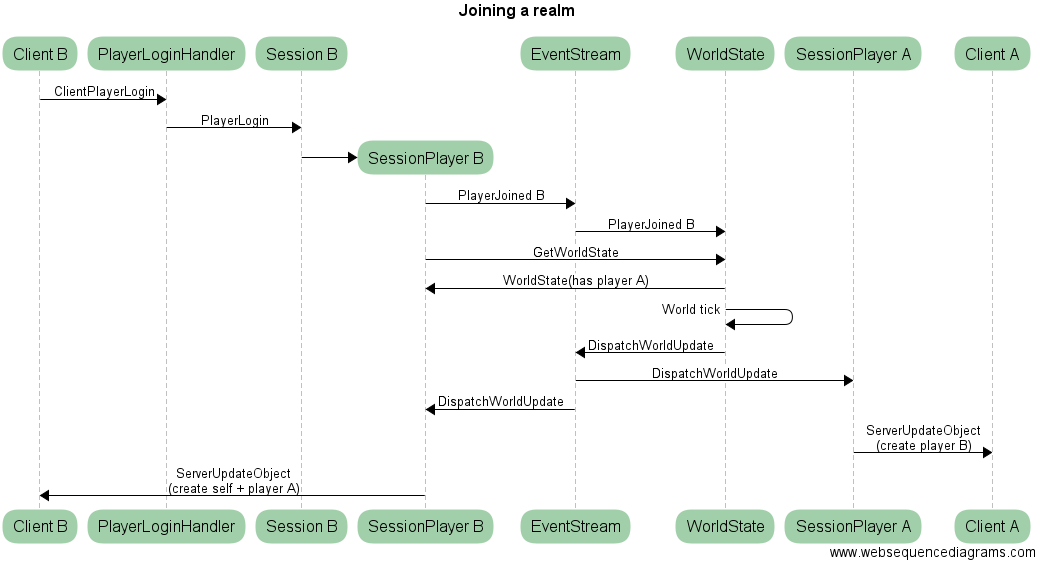
\includegraphics[width=0.95\paperwidth]{playerLogin}
    \caption{Sequence diagram of player B joining the realm}
\end{figure}

When a player has selected its character and joined the world, the
\texttt{ClientPlayerLogin} packet is sent by the client.

The \texttt{PlayerLoginHandler} actor then sends an event to the \texttt{Session}
actor, containing the id of the selected character.
Initially, all features related to the in-game character were handled by the
\texttt{Session} actor.

However, to enforce the single responsibility principle, it was decided to move
this responsibility to a separator actor, \texttt{SessionPlayer} that is created
by the \texttt{Session} actor once the client has selected its player.\\

Upon its creation, the \texttt{SessionPlayer} actor publishes a
\texttt{PlayerJoined} event to the event stream.  
On the next world tick, this event will be a part of the
\texttt{DispatchWorldUpdate} message received by all \texttt{SessionPlayer}
actors (including the sender).

\begin{sloppypar}

From the client's point of view, the loading screen lasts until it receives its
first \texttt{ServerObjectUpdate} packet.
Therefore, if a client has joined the world during the last tick, the contents
of the \texttt{ServerObjectUpdate} packet include:
\begin{itemize}
    \item for the player itself, information about its
        own character, such as its looks, current statistics, initial
        position and all the other players that are already in world
    \item for other players, the packet would contain similar information,
        telling them that a new player has spawned at some position
\end{itemize}

\end{sloppypar}

As a player joining the world must also know about existing players, the
\texttt{SessionPlayer} sends upon creation a \texttt{GetWorldState} message to
the \texttt{WorldState} actor, which answers with a list of players currently in
world.

\subsection{Player movement}

There are various messages in the protocol used for movement.
All of them have the same structure but use a different opcode, indicating what
type of movement is being done.

As the movements require direct handling instead of waiting for the next world
tick, the messages are received by the \texttt{MovementHandler}, adapted for
network lag and directly forwarded to all the clients, by publishing a
\texttt{PlayerMoved} event to the event stream.
The event is received by all \texttt{NetworkWorker} actors, who send the packet
to the client.

Lag compensation is a simple process.
The client regularly (every 10 seconds) synchronizes its local time with the
server's time.
When the packet is emitted by the client, it is tagged with the emission time.
On reception by the server, the difference between the server's time and the
packet's time gives a rough estimation of the time it took for the packet to
travel from the client to the server. 
This difference is added to the packet's time tag before it is sent back to
the clients.

\subsection{Interesting challenges ahead}

The feature set that is currently implemented is very limited, and a lot of the
time was spent on necessary and yet unavoidable boilerplate code or overcoming
the steep learning curve.

The environment of an MMORPG server however offers a lot of potential for
challenging code situations.
For the future of this project, on which we intend to continue to work, we
feel like the following features would be interesting challenges.

\subsubsection{Basic game play features}

While not directly technically complex, adding more game features makes for a
richer environment. In a highly concurrent architecture like ours, and with more
features meaning more data, it is a challenge to design data management in a way
that is both correct (i.e.\ no concurrency issues) and scalable.

These features could be:
\begin{itemize}
    \item Unit fields (required for almost everything else, we managed to avoid
        this complex feature for the duration of the project)
    \item Spell casting
    \item \gls{NPC}
\end{itemize}

These basic features also serve as openings for more technically interesting
features.

\subsubsection{Non playing characters}

Adding non-players characters to the game opens up a lot of interesting
challenges.
Indeed, with many creatures on a map, it would be impossible in the time of a
single world tick to iterate on all of them.
Moreover, it would also be pointless, as a player is limited in the amount of
information it can display on screen.

As such, it is interesting to discuss ways to split up the world in smaller
pieces.
Of course, as the World of Warcraft client and player perceives the world
as one big continuous space, it is not possible to put hard barriers between
these smaller pieces.
A common approach is to layer the world with a grid, where every entity belongs
to a cell. As entities (even creatures) can move freely between different cells 
of the grid, keeping the grid up to date in real time is a task in itself,
specially with a concurrent environment.

Generally speaking, this field of research is known as spatial indices.

\subsubsection{Distributed application}\label{distr}

As it currently stands, our application only benefits from `vertical scaling':
the only way bigger workloads can be handled, ignoring better code, is by using
faster hardware.
For production software, this is insufficient as hardware progress is slow
and costly.

Horizontal scaling means that the application can take advantage of additional
computers.
In our case, Akka supports horizontal scaling: it is possible for an
\texttt{ActorSystem} to be spread amongst multiple machines (Akka Cluster
containing Akka Nodes).
However, it is not automatic and it is the programmer's responsibility to
correctly assign actors to nodes.
Indeed, having actors that communicate a lot on different nodes will incur
serialization and network overhead for every message, which would result in a
loss of performance.\\

As World of Warcraft is an open world that is continuous from the point of view
of the player, isolating groups of actors is difficult.
However, there exists a few hard borders which can be used.
The main one is continents. The main world, in the version we support, is split
in four main continents (named Kalimdor, the Eastern Kingdoms, Northrend and
Outland).

There is little communication between those continents: most actors of a
continent (creatures, various game objects) are created and will always reside
within said continent.

Players can switch continents, but it is not seamless as it requires a loading
screen on the client's side.
Thus, moving a Player's actor from one continent's node to another would
cause little issue.

Certain actions (chat, groups, guilds, instances, battlegrounds\ldots) 
require interacting with a player whose actor is on a different node.
As these actions are not real time, node crossing overhead is not an issue.

One remaining issue is that the client currently uses a single TCP connection,
therefore there has to be a front end server through which all network data
will pass.
For production grade software with actual players, latency added by such a proxy
might matter and would depend on a lot of factors, e.g.\ the cluster's hardware
configuration.

For a technical demonstration such as this project however, this issue can be
ignored.

\subsubsection{Raycasting}

When two entities of the world are interacting with one another, they oftentimes 
must have line of sight on one another.
Concretely, it would not make sense to be able to cast spells on a creature from
behind a wall.
A common problem is knowing who is in line of sight of whom in real time.

Solving this problem implies loading the maps in memory of the world, which in
itself is already complicated due to the associated reverse engineering
challenges.
There are then well-known algorithms to check for line of sight.

An interesting part of this approach would be to split off the actors
responsible for this work to another machine. With a low enough network latency
(e.g. InfiniBand) and a machine with hardware optimized for such
calculations (e.g.\ multiple GPUs if the calculations lend themselves well to
to GPU computing), this design could offer improvements in scalability.

This is also way to open up to the domain of `server-side world physics'.

% \clearpage

\section{Conclusion}

% WoW is major game and complex
% Basing our work off reverse engineered work was a struggle
% We highly enjoyed the opportunity offered by 4MMPF to provide our own topic
% and work on something we liked, while having that work recognized as a
% worthwhile learning endeavour.
% From our code, we are happy with what we have learned in terms of programming,
% but are a bit disappointed with not having been able to reach the distributed
% stage in the provided time frame, as we feel like it would have made our piece
% of software much cooler. We are however still happy with the featureset we have
% implemented and, though we are now still improving our code base (because we
% learned), we feel like we have set a good foundation for more features.

World of Warcraft has been a corner stone of online gaming for years now.
While it was a thrilling experience to work on game we enjoyed so much, it was
certainly not the simplest choice.
Indeed, reverse-engineering, even when done by others, introduces a lot of
uncertainty in otherwise simple tasks.

Far from our minds to back down from difficulty, working in such conditions was
valuable training to further develop our instincts for programming and
more importantly debugging. 

In terms of academia, we highly appreciated the opportunity offered by the
`Specialty project' module to develop an idea of our own from proposal
to final application.
By the same token, we also value the recognition and trust our work receives
when it is acknowledged as a worthwhile learning endeavor by the school's
faculty.

On the topic of the final software, we would have enjoyed being able to fit the
changes described in~\ref{distr}~(\nameref{distr}) in the available time.
We felt those changes would really have brought a sense of closure to the
project, as they would definitely have ticked the `scalability' checkbox.

Nonetheless, we had the occasion to explore many different domains of
computer engineering, from software architecture to cryptography.  We attained
our objectives in terms of featureset, and managed to do so while keeping our
code clean and faithful to its own principles.

On a similar topic, we never waivered in our dedication to writing unit tests
and obtaining peer and continuous integration approval before merges, which
we believe was a factor of success.

Finally, we would like to express our thanks to Mr Franck ROUSSEAU, Blizzard
Entertainement, the World of Warcraft emulation community and all others
involved.

\section{References}

\begingroup{}
\renewcommand{\section}[2]{}%
\begin{thebibliography}{9}
    \bibitem{Scala API documentation}
    Scala API documentation,
    \url{https://www.scala-lang.org/api/current/}

    \bibitem{Akka API documentation}
    Akka API documentation,
    \url{http://doc.akka.io/docs/akka/current/scala.html}

    \bibitem{scodec API documentation}
    scodec API documentation,
    \url{http://scodec.org/api/scodec-core/1.9.0/}

    \bibitem{FastClasspathScanner documentation}
    FCP documentation,
    \url{https://github.com/lukehutch/fast-classpath-scanner/wiki}

    \bibitem{TrinityCore} 
    TrinityCore,
    \url{https://www.trinitycore.org/}

\end{thebibliography}
\endgroup{}

\end{document}
